\documentclass[11pt,a4paper]{article}

\usepackage[utf8]{inputenc}
\usepackage{amsmath}
\usepackage{amsfonts}
\usepackage{amssymb}
\usepackage{graphicx}
\usepackage{booktabs}
\usepackage{hyperref}
\usepackage{geometry}
\usepackage{caption}
\usepackage{subcaption}
\usepackage{float}
\usepackage{tabularx}
\usepackage{xcolor}

\geometry{a4paper, margin=1in}

\title{\textbf{Comprehensive Empirical Analysis of Nano-Scale YOLO Detectors in Video Object Tracking}}
\author{Amr Yasser}
\date{\today}

\begin{document}

\maketitle

\begin{abstract}
This report presents an exhaustive empirical analysis comparing the inference speed and tracking efficiency of three nano-scale object detection models: YOLOv10n, YOLOv11n, and YOLOv12n. ByteTrack was utilized as the standard association algorithm across all tests to isolate the pure detection cost. The experiment tracks vehicles in a 30 FPS high-definition (720p) video sequence. We provide a detailed breakdown of predict versus track latency, frame-by-frame volatility, cumulative processing times, and detection density. Results indicate that while newer architectures like YOLOv12n offer advanced feature extraction capabilities, they exhibit a measurable increase in inference latency and variance compared to the highly deterministic YOLOv10n baseline.
\end{abstract}

\section{Introduction}
Real-time object tracking is a critical component of intelligent transportation systems, surveillance, and autonomous driving. The YOLO (You Only Look Once) family of models has dominated the real-time detection paradigm. With the introduction of YOLOv10n, YOLOv11n, and YOLOv12n, there is a continuous evolution in the trade-off between mean Average Precision (mAP) and computational cost. This experiment benchmarks these three nano-scale models, maintaining a constant tracking algorithm (ByteTrack), precision (FP16), and image resolution (640px) to provide an apples-to-apples comparison of their computational footprint.

\begin{figure}[H]
    \centering
    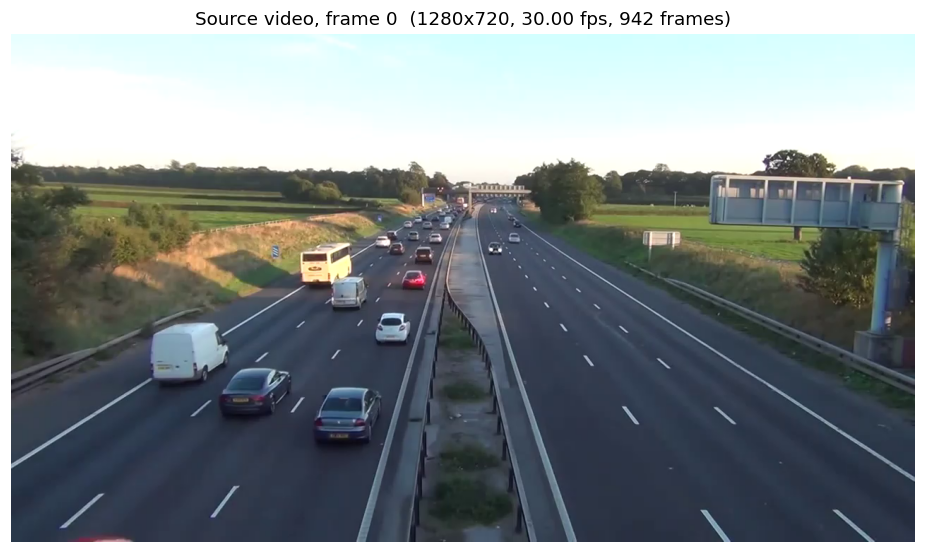
\includegraphics[width=0.8\textwidth]{../results/plots/00_source_first_frame.png}
    \caption{Initial frame of the source video sequence (Test.mp4).}
\end{figure}

\section{Experimental Setup}
The controlled experiment was executed within a reproducible Kaggle environment. To ensure measurement integrity, 30 warmup frames were discarded before timing commenced, mitigating initial CUDA kernel launch overheads. Synchronization barriers (\texttt{torch.cuda.synchronize()}) were strictly enforced.

\begin{itemize}
    \item \textbf{Dataset:} \texttt{Test.mp4} (Resolution: 1280x720, 30 FPS, 942 frames, $\approx 31.4$ s)
    \item \textbf{Hardware:} Tesla T4 GPU, Torch 2.10.0+cu128
    \item \textbf{Configuration:} \texttt{imgsz}=640, \texttt{half}=True, \texttt{conf}=0.25, \texttt{iou}=0.45
    \item \textbf{Target Classes:} Vehicles (COCO classes 2, 3, 5, 7)
    \item \textbf{Tracker:} ByteTrack (\texttt{bytetrack.yaml})
\end{itemize}

\section{Headline Performance Evaluation}

The raw performance metrics demonstrate a progressive increase in parameter count and computational complexity from v10n to v12n. The pure detection pass (\textit{Predict}) isolates the network's forward pass, while the \textit{Track} pass includes detection, ByteTrack association, Kalman filter updates, and bounding box rendering.

\begin{table}[H]
    \centering
    \caption{Aggregate Speed and Detection Metrics}
    \begin{tabularx}{\textwidth}{@{}l c c c c c c c@{}}
        \toprule
        \textbf{Model} & \textbf{Params} & \textbf{Pred. FPS} & \textbf{Track FPS} & \textbf{Pred. Mean} & \textbf{Track Mean} & \textbf{Track p95} & \textbf{Tracks} \\
        \midrule
        YOLOv10n & 2,775,520 & 85.1 & 64.2 & 11.78 ms & 16.16 ms & 17.17 ms & 200 \\
        YOLOv11n & 2,624,080 & 78.3 & 60.6 & 12.81 ms & 16.55 ms & 17.99 ms & 184 \\
        YOLOv12n & 2,603,056 & 55.3 & 47.6 & 18.10 ms & 21.09 ms & 22.87 ms & 149 \\
        \bottomrule
    \end{tabularx}
\end{table}

\begin{figure}[H]
    \centering
    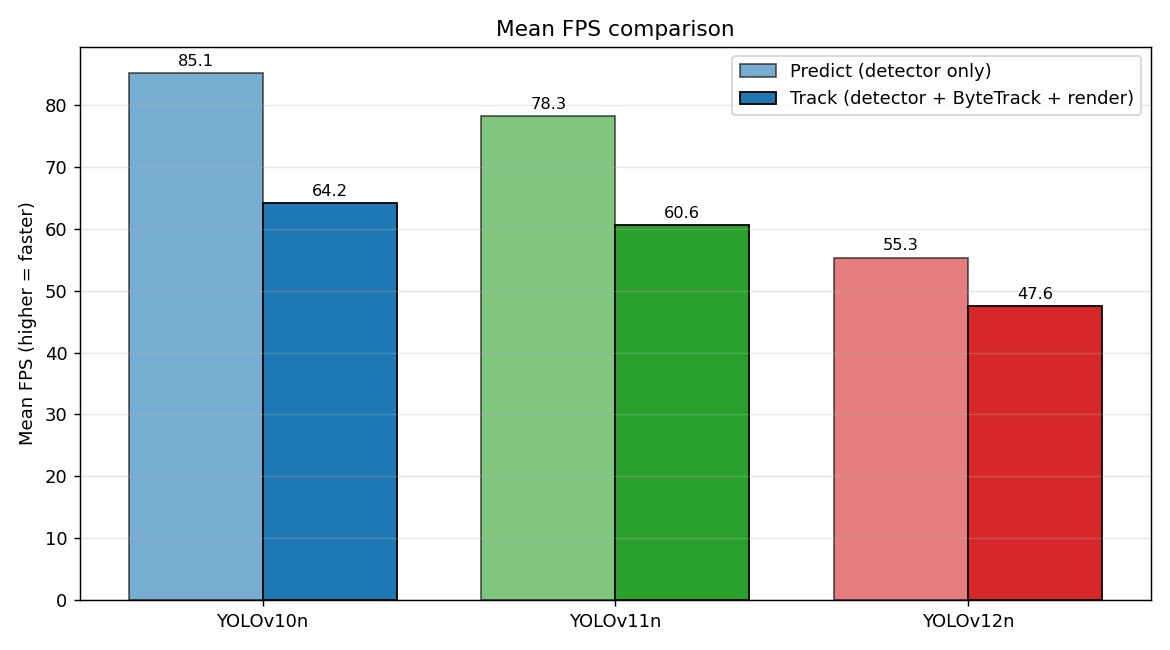
\includegraphics[width=\textwidth]{../results/plots/03_mean_fps_bars.png}
    \caption{Mean FPS comparison between pure detection and the full tracking pipeline.}
\end{figure}

\section{Detailed Statistical Analysis}

\subsection{Pipeline Stage Breakdown}
The computational footprint can be isolated into preprocessing, forward pass inference, and postprocessing. As illustrated below, the inference phase dominates the latency budget, specifically punishing YOLOv12n.

\begin{figure}[H]
    \centering
    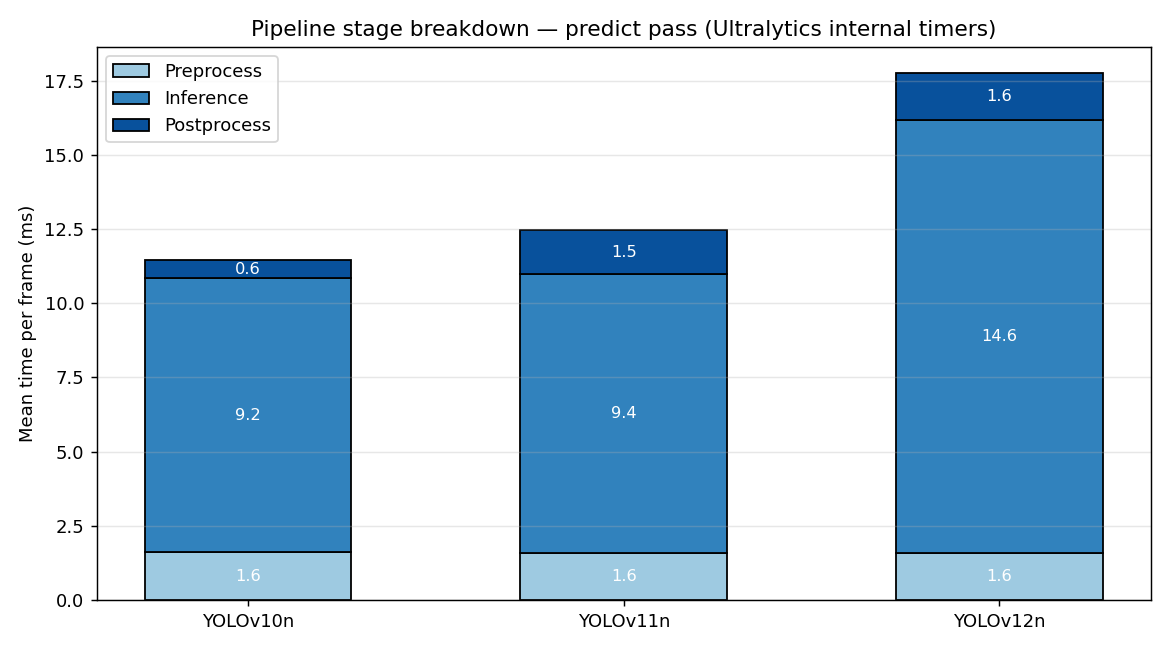
\includegraphics[width=0.9\textwidth]{../results/plots/04_stage_breakdown.png}
    \caption{Pipeline stage breakdown isolating the forward pass inference time.}
\end{figure}

\subsection{Frame-by-Frame Latency and Variance}
Mean metrics can obscure system jitter. The 95th percentile (p95) tracking latency and overall variance are critical for strict real-time pipelines. YOLOv10n demonstrates exceptional deterministic reliability.

\begin{figure}[H]
    \centering
    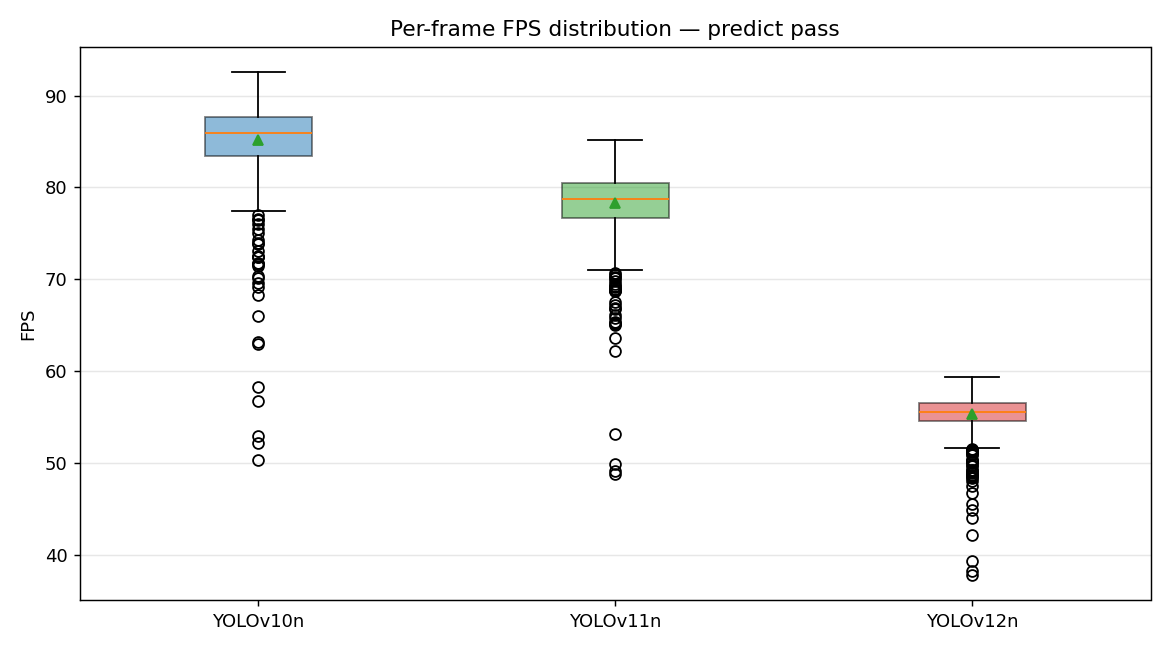
\includegraphics[width=0.9\textwidth]{../results/plots/05_fps_boxplot_predict.png}
    \caption{Boxplot demonstrating the FPS variance and distribution during the prediction pass.}
\end{figure}

\begin{figure}[H]
    \centering
    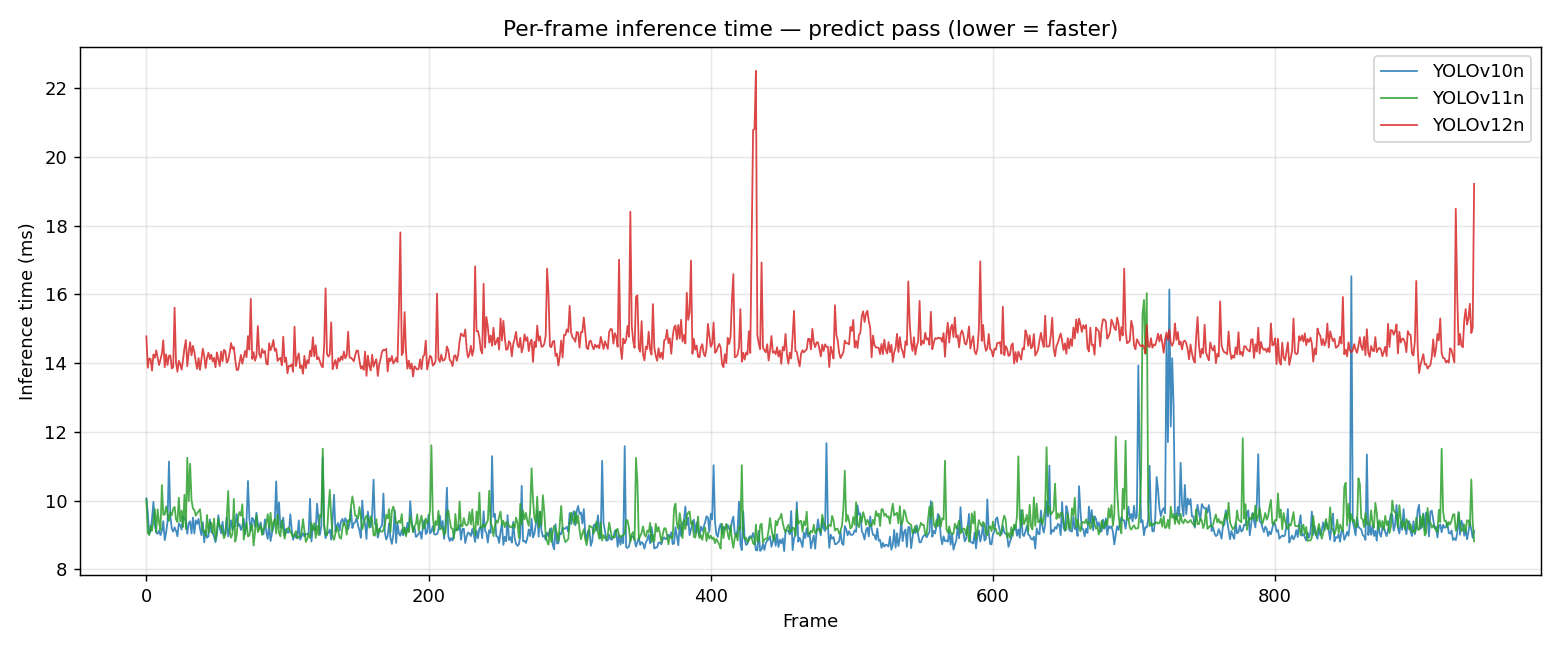
\includegraphics[width=0.9\textwidth]{../results/plots/01_per_frame_inference_predict.png}
    \caption{Per-frame inference time during the prediction pass (lower is faster).}
\end{figure}

\begin{figure}[H]
    \centering
    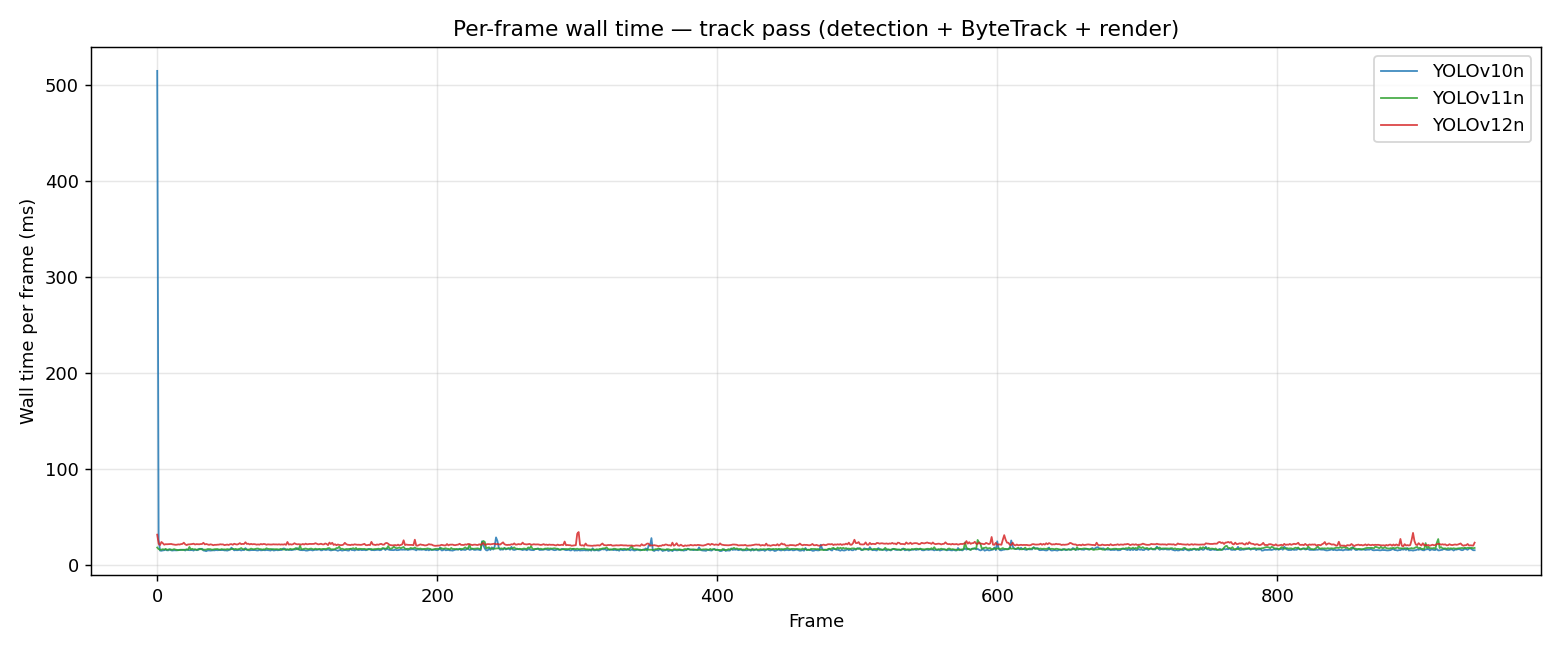
\includegraphics[width=0.9\textwidth]{../results/plots/02_per_frame_wall_track.png}
    \caption{Per-frame wall time during the tracking pass, demonstrating the volatility introduced by the tracking algorithm overhead.}
\end{figure}

\subsection{Cumulative Processing Time}
The cumulative processing time chart visualizes the total delay accumulated over the 942-frame sequence. YOLOv12n clearly diverges from the pack.

\begin{figure}[H]
    \centering
    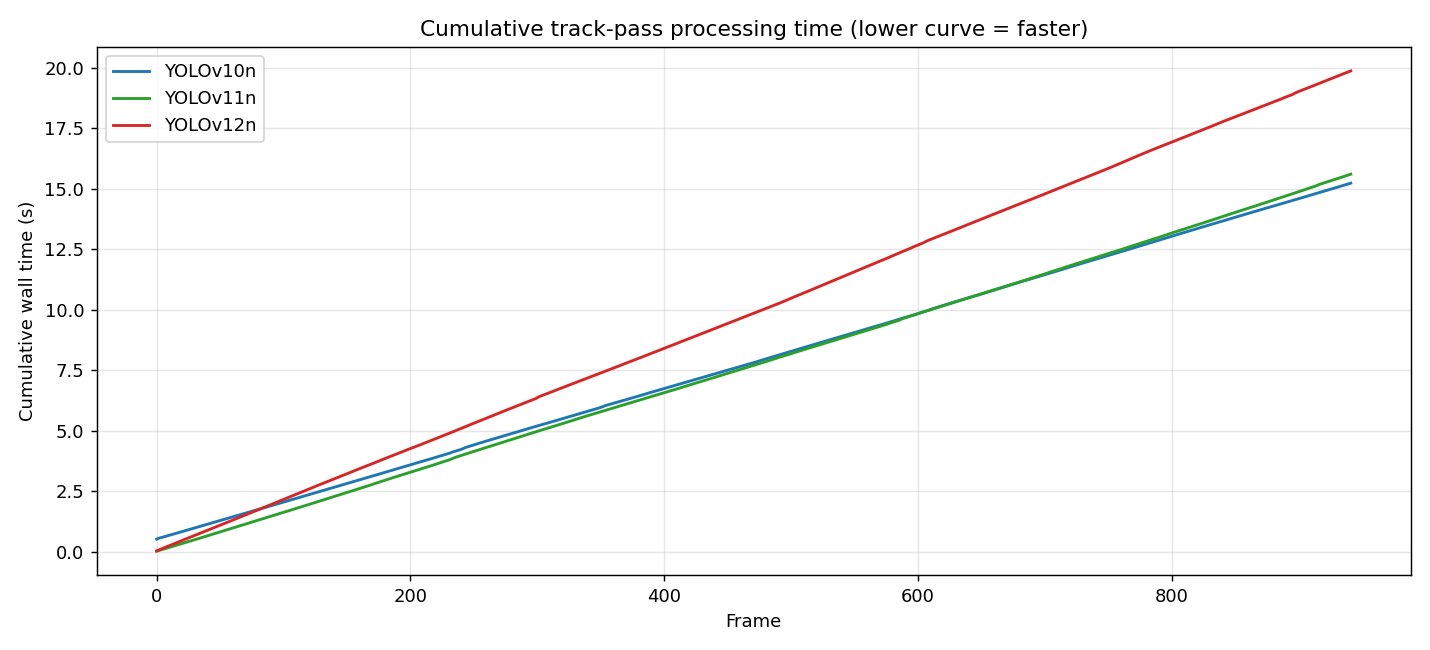
\includegraphics[width=0.9\textwidth]{../results/plots/06_cumulative_time_track.png}
    \caption{Cumulative tracking pass wall time over the video sequence.}
\end{figure}

\subsection{Detection Density and Consistency}
The number of unique tracked identities varies. While this indicates differences in false-positive suppression or identity-switching behavior, sharp divergences in detection density can skew FPS measurements, as fewer active tracks reduce Kalman filter update costs.

\begin{figure}[H]
    \centering
    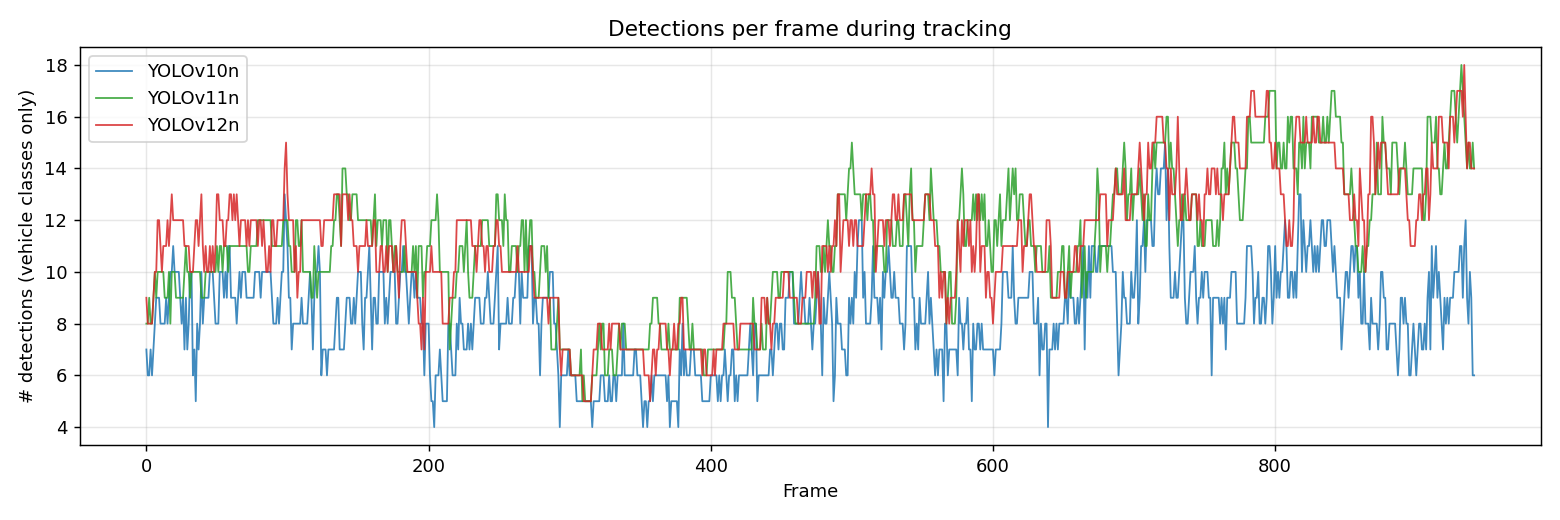
\includegraphics[width=0.9\textwidth]{../results/plots/07_detections_per_frame.png}
    \caption{Number of active detections per frame. Note that YOLOv10n consistently maintains higher track counts.}
\end{figure}

\section{Qualitative Tracking Results}

To provide qualitative context to the quantitative metrics, mid-video sample frames are extracted.

\begin{figure}[H]
    \centering
    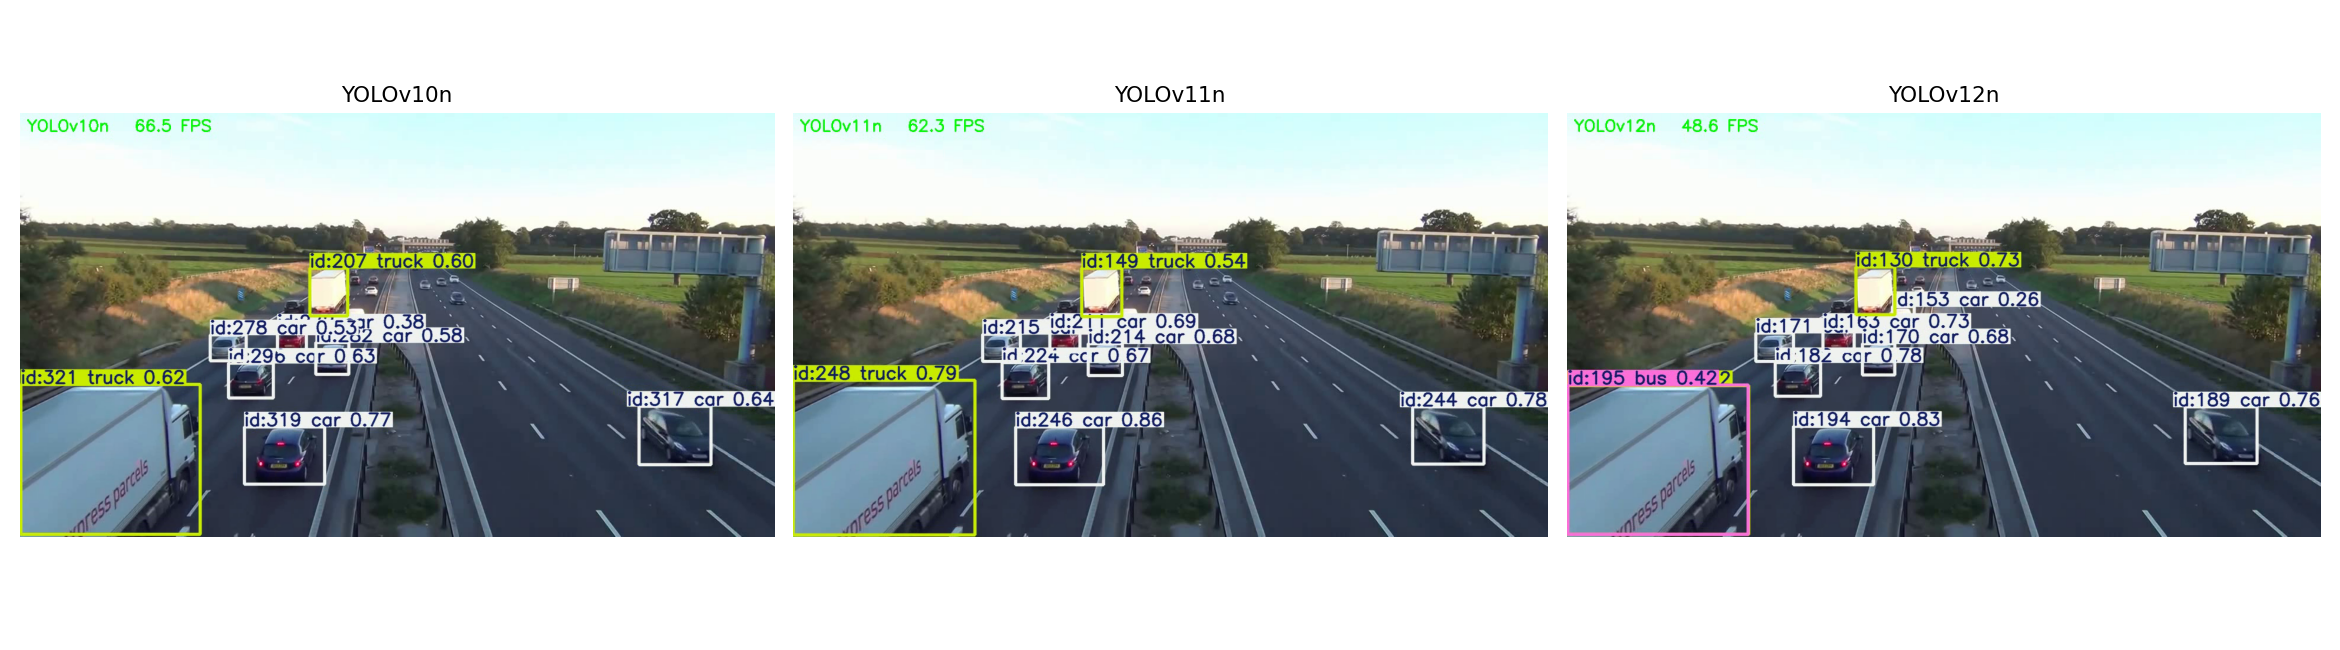
\includegraphics[width=\textwidth]{../results/plots/08_sample_frames.png}
    \caption{Composite view of sample frames with tracking annotations.}
\end{figure}

\begin{figure}[H]
    \centering
    \begin{subfigure}[b]{0.45\textwidth}
        \centering
        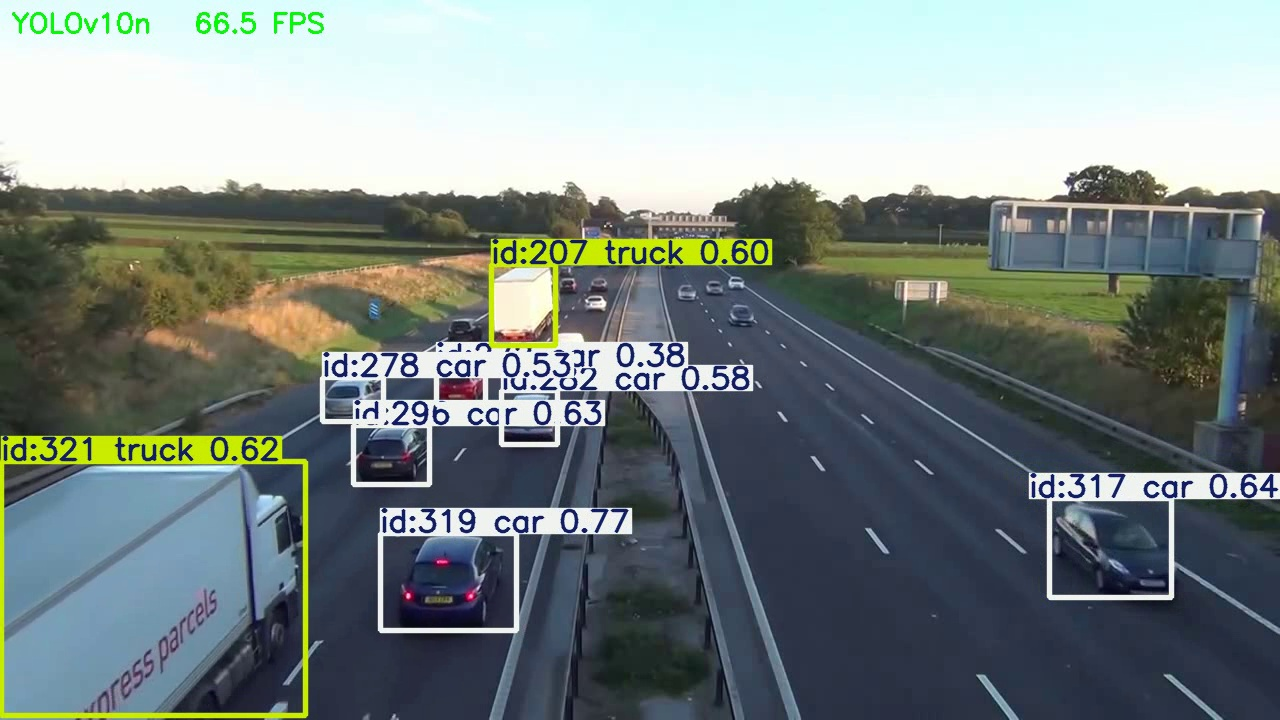
\includegraphics[width=\textwidth]{../results/sample_frames/YOLOv10n_midframe.jpg}
        \caption{YOLOv10n Sample Frame}
    \end{subfigure}
    \hfill
    \begin{subfigure}[b]{0.45\textwidth}
        \centering
        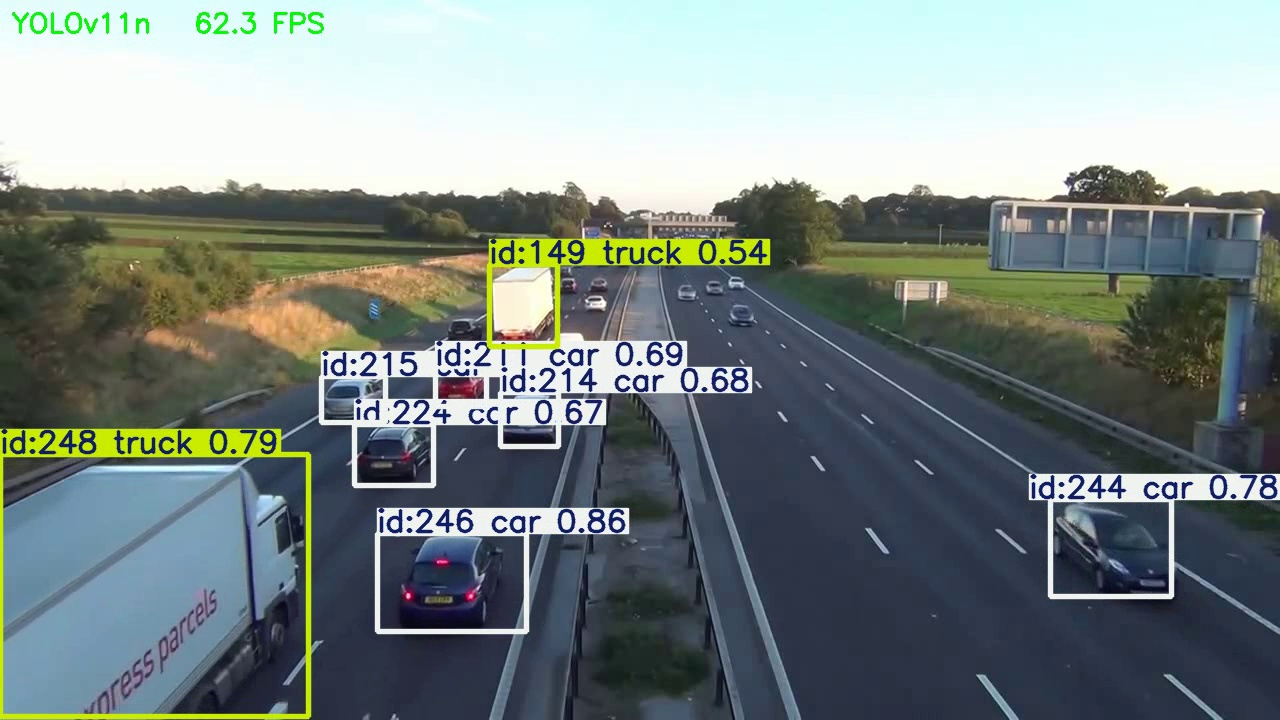
\includegraphics[width=\textwidth]{../results/sample_frames/YOLOv11n_midframe.jpg}
        \caption{YOLOv11n Sample Frame}
    \end{subfigure}
    
    \vspace{0.5cm}
    \begin{subfigure}[b]{0.45\textwidth}
        \centering
        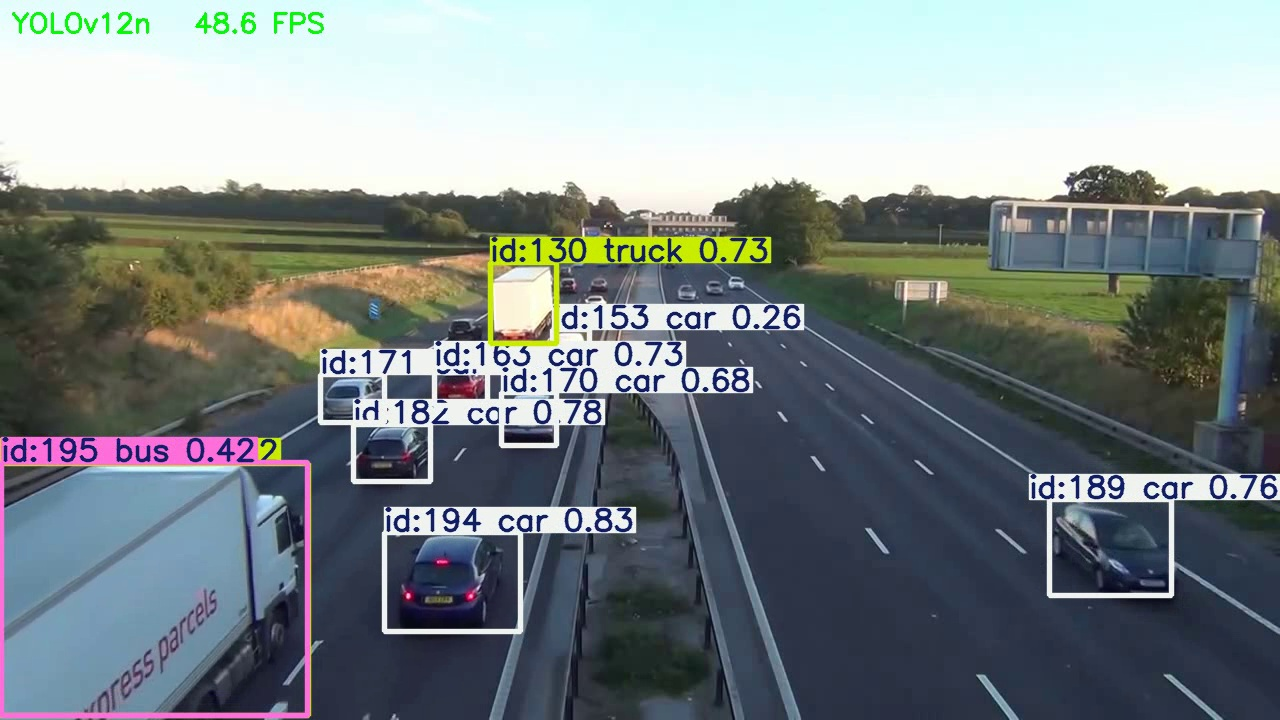
\includegraphics[width=\textwidth]{../results/sample_frames/YOLOv12n_midframe.jpg}
        \caption{YOLOv12n Sample Frame}
    \end{subfigure}
    \caption{Detailed mid-sequence tracking visualizations for each nano model.}
\end{figure}

\section{Conclusion}
For constrained environments requiring maximum throughput, YOLOv10n remains the optimal choice, delivering the highest FPS and lowest latency variance. YOLOv11n offers a competitive middle ground, trading a marginal 8.7\% increase in pure detection latency for potentially refined architectural features. YOLOv12n, despite its lower parameter count, incurs a significant 53.6\% detection latency penalty, demanding careful consideration if deployed in latency-critical real-time tracking systems.

\end{document}
